\documentclass{classrep}
\usepackage[utf8]{inputenc}
\usepackage{color}
\usepackage{lmodern}
\usepackage{graphicx}

\DeclareUnicodeCharacter{00A0}{~}

\studycycle{Informatyka, studia dzienne, inż I st.}
\coursesemester{VI}

\coursename{Sztuczna inteligencja i systemy ekspertowe}
\courseyear{2020/2021}

\courseteacher{dr inż. Krzysztof Lichy}
\coursegroup{poniedziałek, 10:15}

\author{
  \studentinfo{Paweł Guzek}{224304} \and
  \studentinfo{Krzysztof Szcześniak}{224434} \and
  \studentinfo{Michał Maksajda}{224369} \and
  \studentinfo{Dominik Kasierski}{224323}  
}

\title{Zadanie 1: Piętnastka}

\begin{document}
\maketitle
\pagebreak

\section{Cel}
{\color{black}
Zadanie składało się z dwóch części: programistycznej oraz badawczej. Pierwsza część polegała na napisaniu programu, który znajduje rozwiązanie gry logicznej “Piętnastka”. Badania, które należało przeprowadzić w drugiej części zadania, miały wykazać jak wybrane algorytmy radzą sobie z rozwiązywaniem wskazanej łamigłówki.
}


\section{Wprowadzenie}
{\color{black}
Piętnastka to układanka, która jest reprezentowana przez planszę o rozmiarze 4x4. Plansza jest wypełniona przez 15 płytek, każda z nich ma przypisany numer z zakresu od 1 do 15. Jedno miejsce na planszy zawsze musi pozostać puste. Warunkiem końcowym tej gry logicznej jest ułożenie wszystkich 15 płytek, tak aby numery na nich zawarte były ułożone w kolejności rosnącej.

Algorytmy, które zostały wykorzystane w części badawczej:
\begin{itemize}
  \item DFS (Depth-first Search) - przejście grafu w głąb. Trawersowanie polega w tym przypadku na przechodzeniu kolejno lewego oraz prawego poddrzewa. 
Z węzła początkowego (korzenia), następuje przejście do pierwszego połączonego z nim węzła - przyjmijmy, że jest to węzeł B (rys. 1). Z węzła B przechodzimy do pierwszego nie odwiedzonego węzła, który jest bezpośrednio połączony z węzłem B. W sytuacji, kiedy nie istnieje nieodwiedzony węzeł, następuje powrót do poprzedniego węzła, a czynność zostaje powtórzona do momentu odwiedzenia wszystkich węzłów.

\begin{figure}[ht!]
	\begin{center}
		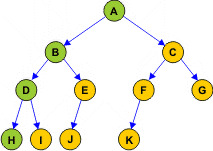
\includegraphics[scale=0.5]{dfs_tree}
		\caption{DFS - kolejność odwiedzania stanów}
	\end{center}
\end{figure}

  \item BFS (Breadth-first Search) - Algorytm przeszukiwania wszerz
Algorytm rozpoczyna generowanie sąsiadów od stanu początkowego (korzenia), następnie (w kolejności wybranej przez użytkownika) odwiedza wygenerowane stany oraz generuje sąsiadów dla nich. W pierwszej kolejności odwiedzani są sąsiedzi znajdujący się w tej samej odległości od korzenia. Po odwiedzeniu wszystkich elementów o tej samej odległości, następuje przejście do kolejnego poziomu oraz odwiedzanie względem kolejności wygenerowania.

\begin{figure}[ht!]
	\begin{center}
		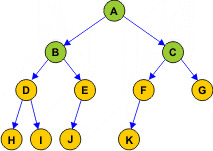
\includegraphics[scale=0.5]{bfs_tree}
		\caption{BFS - kolejność odwiedzania stanów}
	\end{center}
\end{figure}
\newpage

  \item A* - algorytm heurystyczny wykorzystywany do znajdowania ścieżki pomiędzy węzłami w grafie. Zasada działania opiera się na przeszukiwaniu węzłów według wartości funkcji f(x) o wzorze:\\ \centerline{ f(x) = g(x) + h(x), gdzie: }\\ g(x) to funkcja kosztu,\\ h(x) to funkcja heurystyczna.\\ Pierwszeństwo przeszukiwania zostaje wyznaczone dla węzła, który posiada najmniejszą wartość funkcji f(x).
Do przeprowadzenia części badawczej z wykorzystywania algorytmu A* zostały wybrane dwie heurystyki:
  \begin{itemize}
  \item Metryka Hamminga - polega na zliczeniu elementów układanki, które w danym ustawieniu na planszy są umiejscowione w nieprawidłowych miejscach (ich pozycja różni się od pozycji w układzie finalnym - wzorcowym).
  \item Metryka Manhattan - polega na obliczeniu odległości, która dzieli pozycję elementu na planszy w danym ustawieniu, od jej pozycji na planszy w układzie wzorcowym - rozwiązaniu układu.
  \end{itemize}
\end{itemize}

}

\section{Opis implementacji}
{\color{black}
Program jest aplikacją konsolową napisaną w języku Python. Do uruchomienia wymagane jest przekazanie do programu parametrów takich jak:
  \begin{itemize}
  \item akronim strategii użytej do rozwiązania układu,
  \item dodatkowy parametr uszczegóławiający wybraną strategię,
  \item nazwa pliku zawierającego początkowy stan układanki,
  \item nazwa pliku do którego zostanie zapisane rozwiązanie układu,
  \item nazwa pliku do którego zostaną zapisane dodatkowe informacje.
  \end{itemize}
Podczas uruchomienia programu dla układu wejściowego sprawdzane jest czy istnieje dla niego rozwiązanie. Jeżeli rozwiązanie istnieje, za pomocą fabryki SolverFactory tworzony jest obiekt algorytmu rozwiązującego układ oraz następuje próba jego rozwiązania. Układy wczytywane są do klasy Board reprezentującej układ puzzli na planszy. Klasa State odpowiada za przechowywanie informacji dotyczących stanu dla wygenerowanych plansz, zawiera pola takie jak: głębokość rozwiązania, ostatni ruch, czy stan rodzica.

\begin{figure}[ht!]
	\begin{center}
		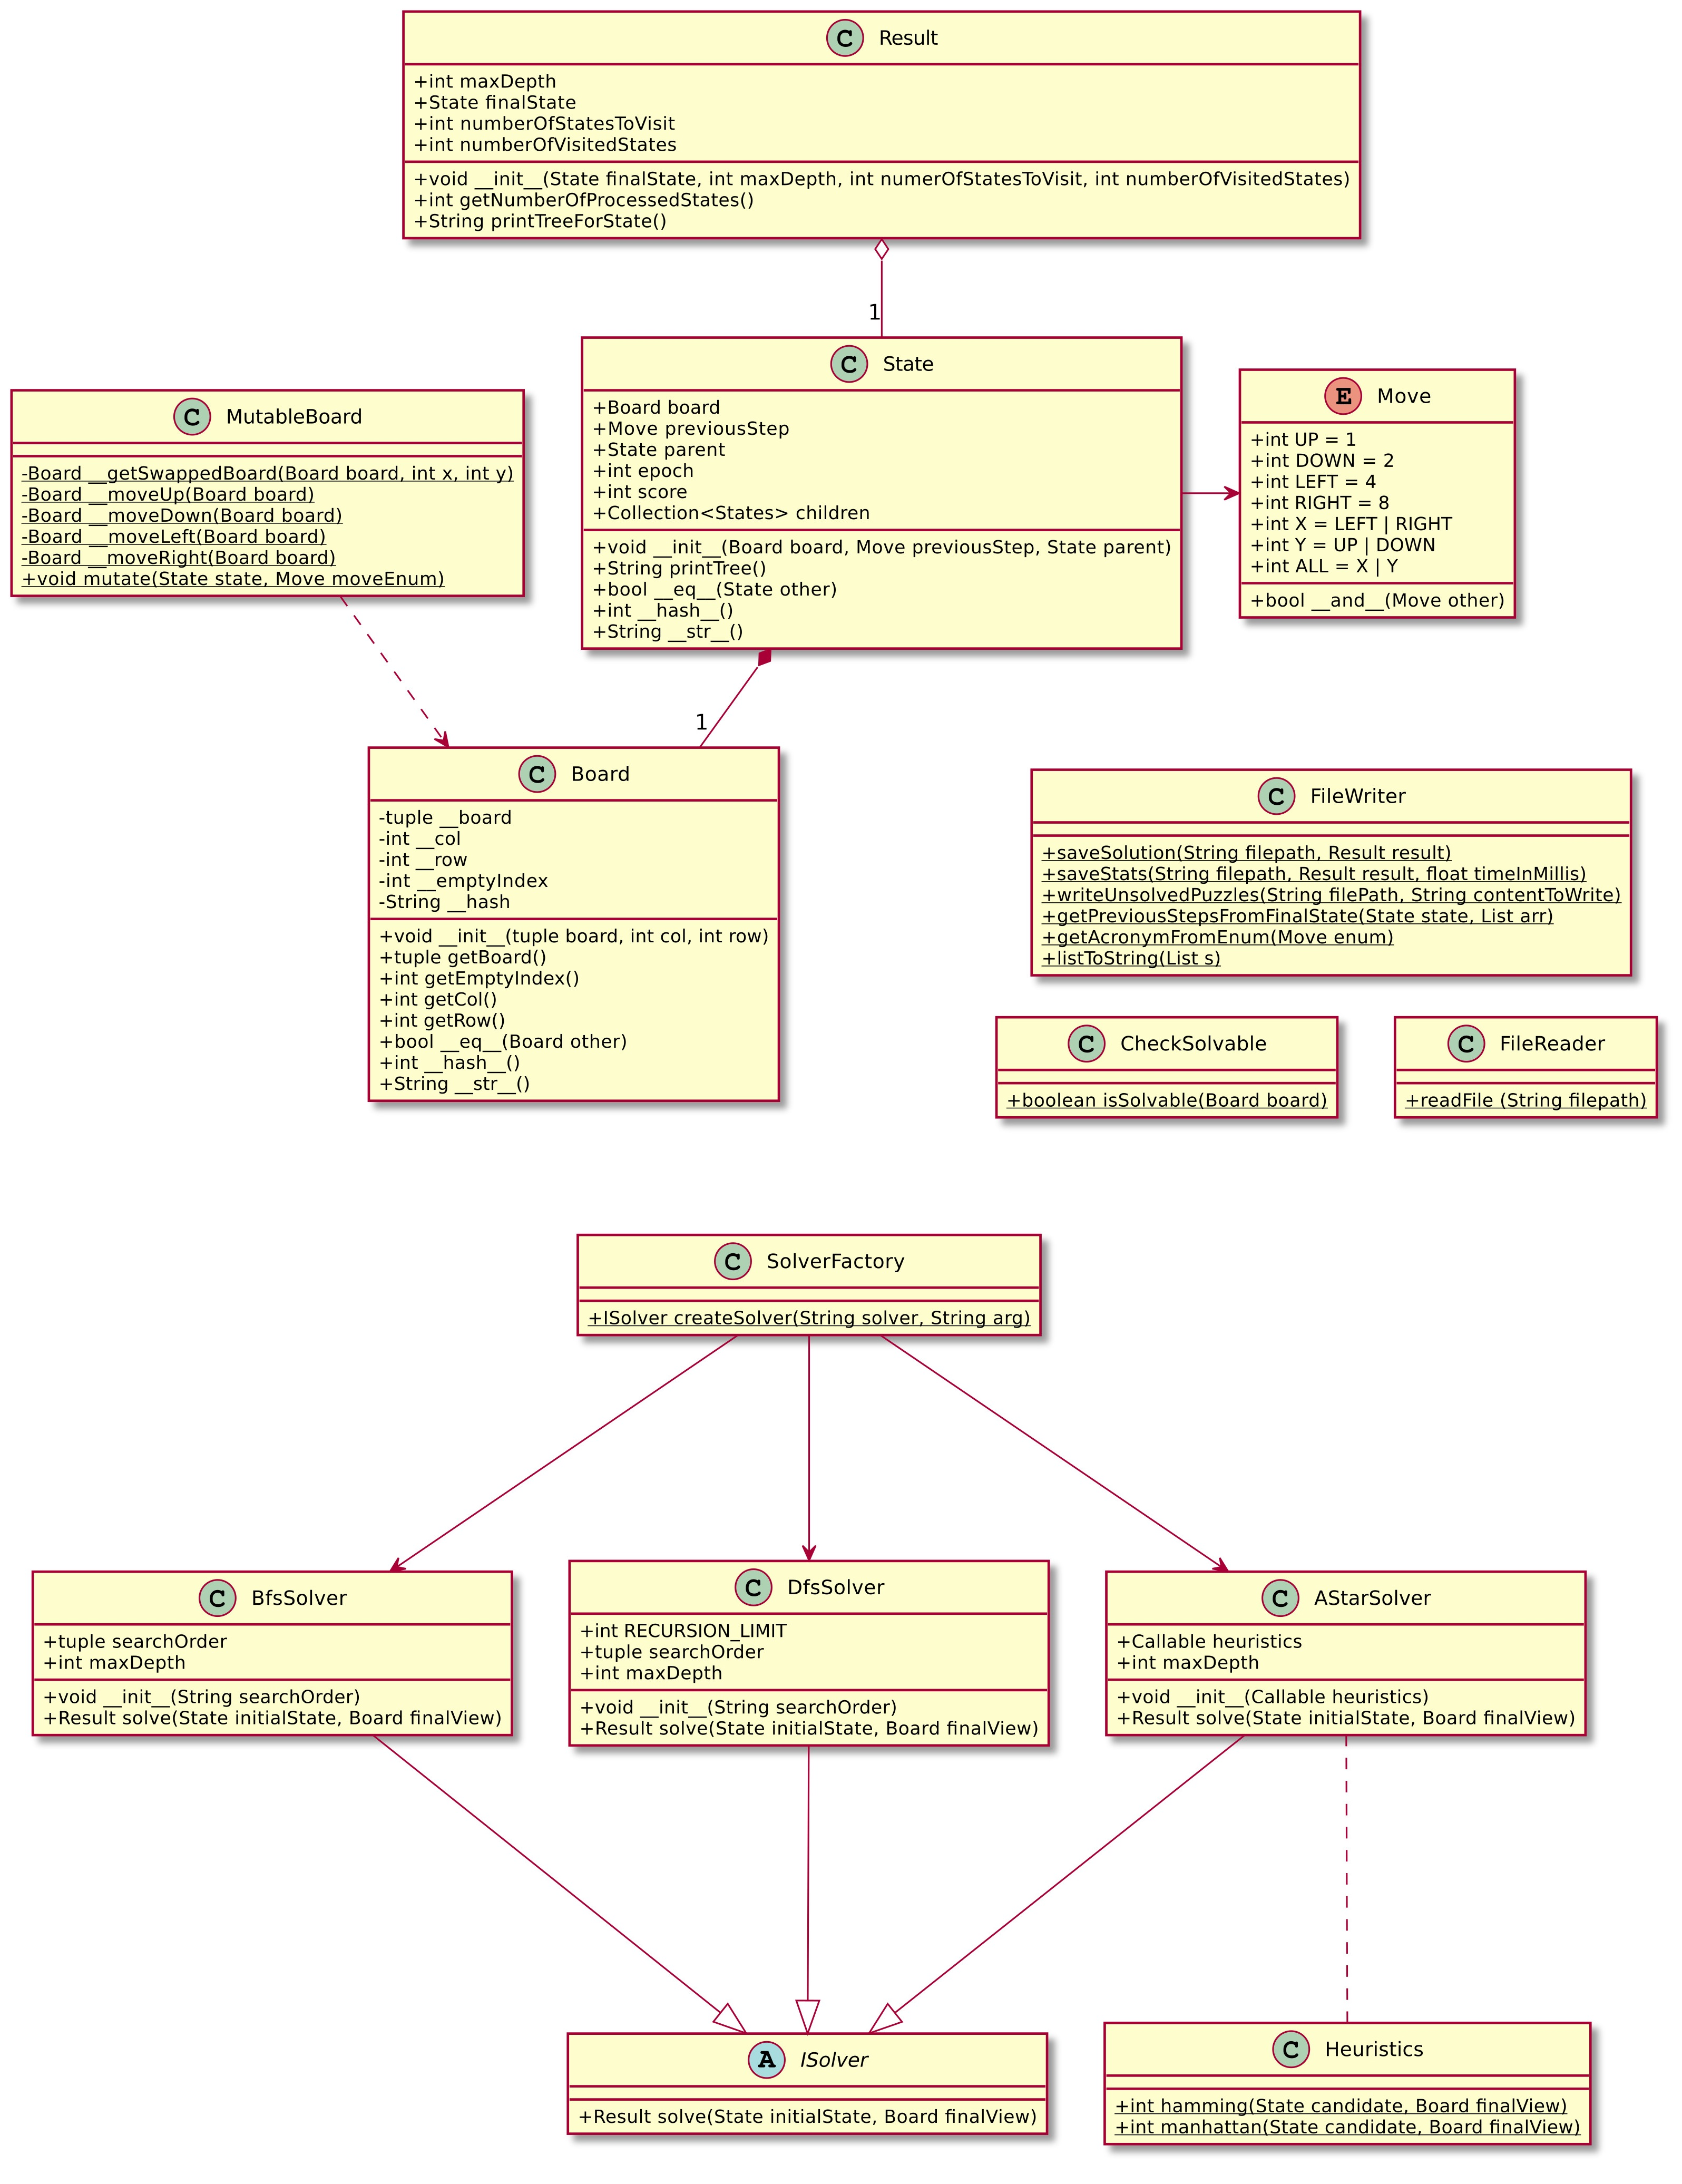
\includegraphics[scale=0.5]{uml}
		\caption{Diagram UML}
	\end{center}
\end{figure}
\newpage

Opis zaimplementowanych strategii:
  \begin{itemize}
  \item BFS - Algorytm przeszukiwania wszerz \\Do zachowania odpowiedniej kolejności przy przechodzeniu pomiędzy stanami zastosowano obiekt (deque) implementujący zachowanie kolejka FIFO.
  \item DFS - Algortym przeszukiwania w głąb \\W celu zachowania odpowiedniej kolejności przy przechodzeniu pomiędzy stanami wykorzystano obiekt (LifoQueue) implementujący zachowanie kolejki LIFO.\\
  \item A* \\Zachowanie odpowiedniej kolejności przy przechodzeniu pomiędzy stanami zostało zrealizowane za pomocą sortowania rosnąco listy dwukierunkowej (deque) implementującej zachowanie kolejki FIFO.
  \end{itemize}
}

\section{Materiały i metody}
{\color{black}
W celu przeprowadzenia badań, których wyniki zamieszczone są w następnej sekcji, wykorzystano narzędzia udostępnione na platformie WIKAMP. Skorzystano z generatora układanek, skryptu generującego pliki rozwiązań, walidatora rozwiązań oraz skryptu ekstraktującego pozyskane dane do jednego pliku. Uzyskane w ten sposób wyniki przetworzono i zobrazowano na wykresach, aby jak najdokładniej przedstawić różnice między wykorzystywanymi algorytmami.}

\section{Wyniki}
{\color{black}
Poniżej zamieszczono wykresy przedstawiające: 
\begin{itemize}
  \item średnią długość rozwiązania,
  \item średnią liczbę stanów odwiedzonych,
  \item średnią liczbę stanów przetworzonych,
  \item średnią maksymalnych głębokości rekursji,
  \item średni czas trwania procesu obliczeniowego.\\
\end{itemize}
Przebadany został każdy algorytm. Uwzględniono porządek przeszukiwania sąsiedztwa bieżącego stanu dla algorytmów BFS i DFS oraz używaną heurystykę dla algorytmu A*.
\newpage

\begin{figure}[ht!]
	\begin{center}
		\vspace{0.3in}
		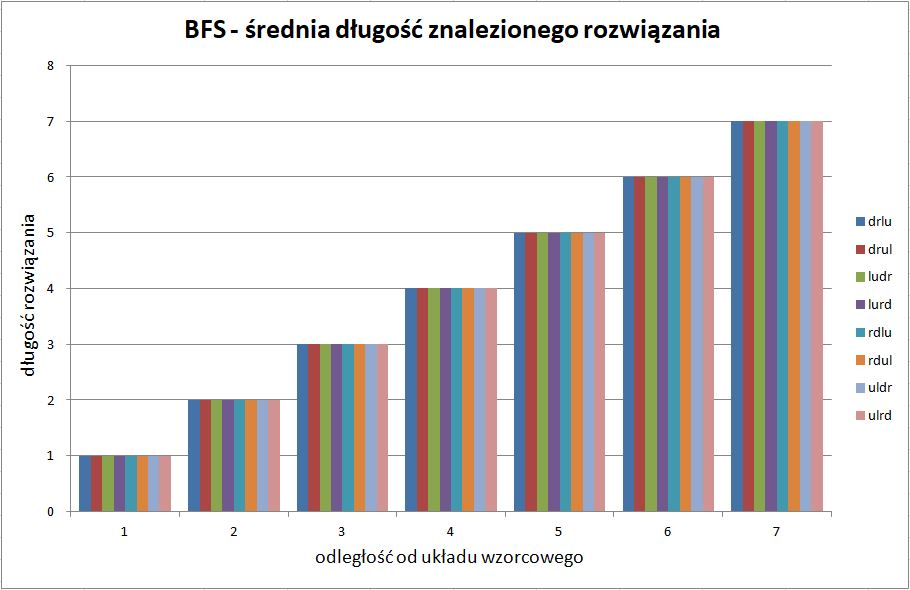
\includegraphics[scale=0.6]{bfs1}
		\caption{BFS - średnia długość znalezionego rozwiązania}
		\vspace{0.5in}
		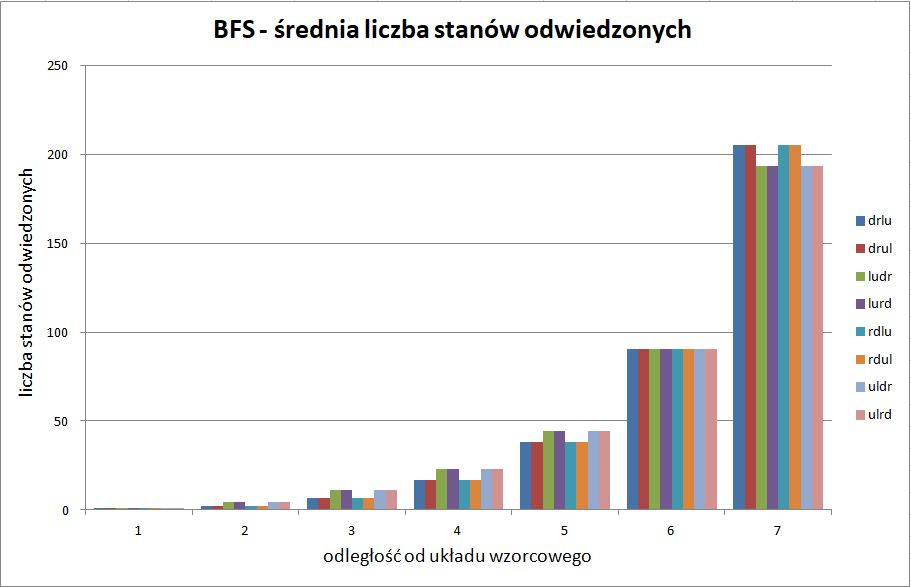
\includegraphics[scale=0.6]{bfs2}
		\caption{BFS - średnia liczba stanów odwiedzonych}
	\end{center}
\end{figure}
\newpage
\begin{figure}[ht!]
	\begin{center}
		\vspace{0.3in}
		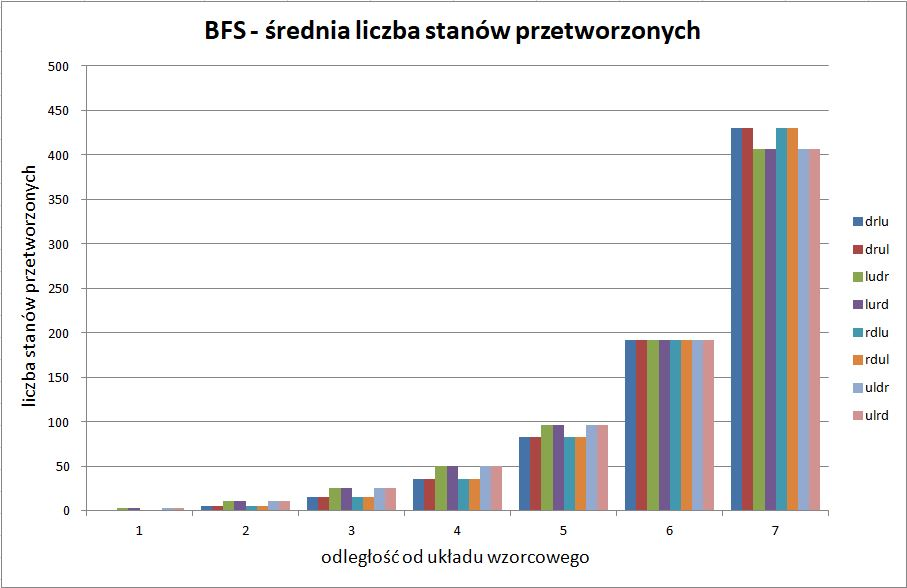
\includegraphics[scale=0.6]{bfs3}
		\caption{BFS - średnia liczba stanów przetworzonych}
		\vspace{0.5in}
		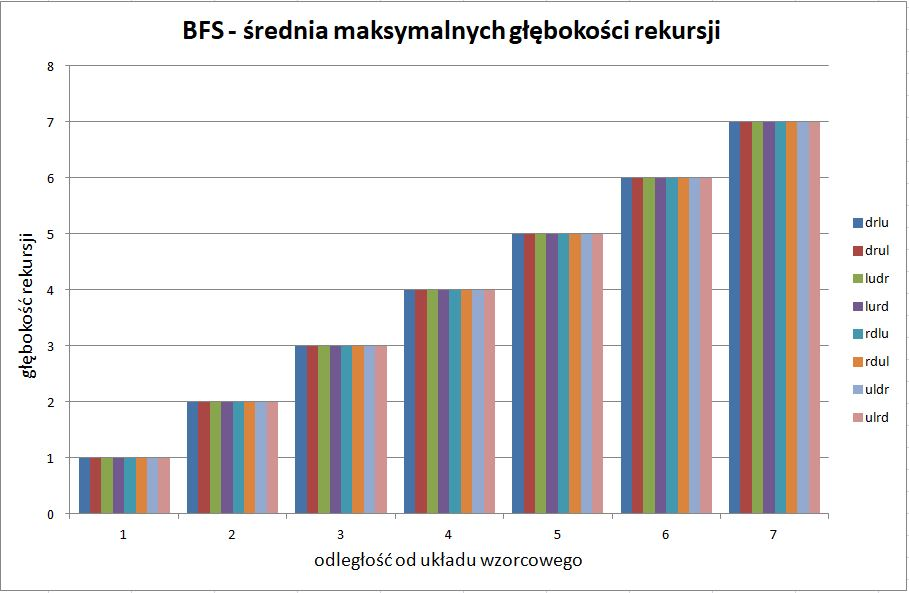
\includegraphics[scale=0.6]{bfs4}
		\caption{BFS - średnia maksymalnych głębokości rekursji}
	\end{center}
\end{figure}
\newpage
\begin{figure}[ht!]
	\begin{center}
		\vspace{0.3in}
		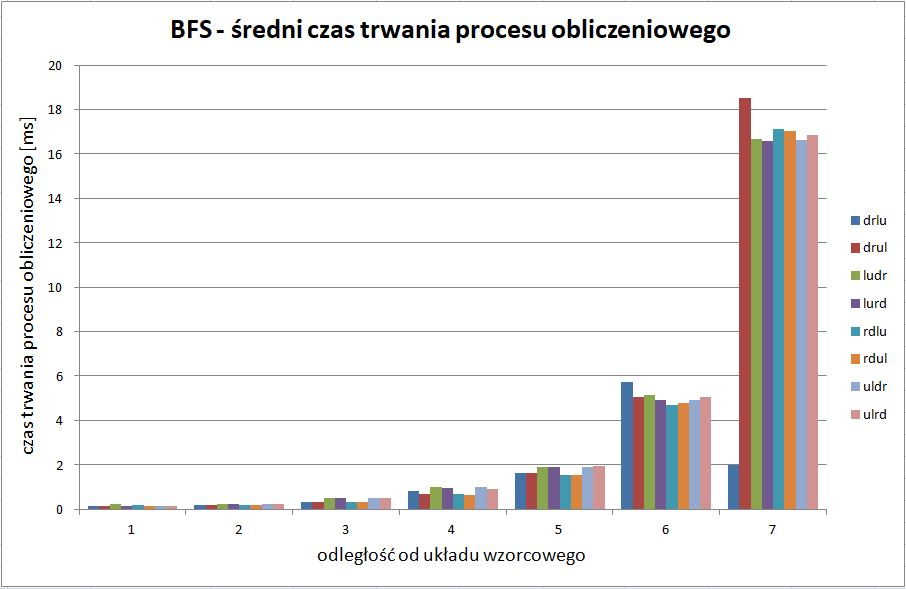
\includegraphics[scale=0.6]{bfs5}
		\caption{BFS - średni czas trwania procesu obliczeniowego}
		\vspace{0.5in}
		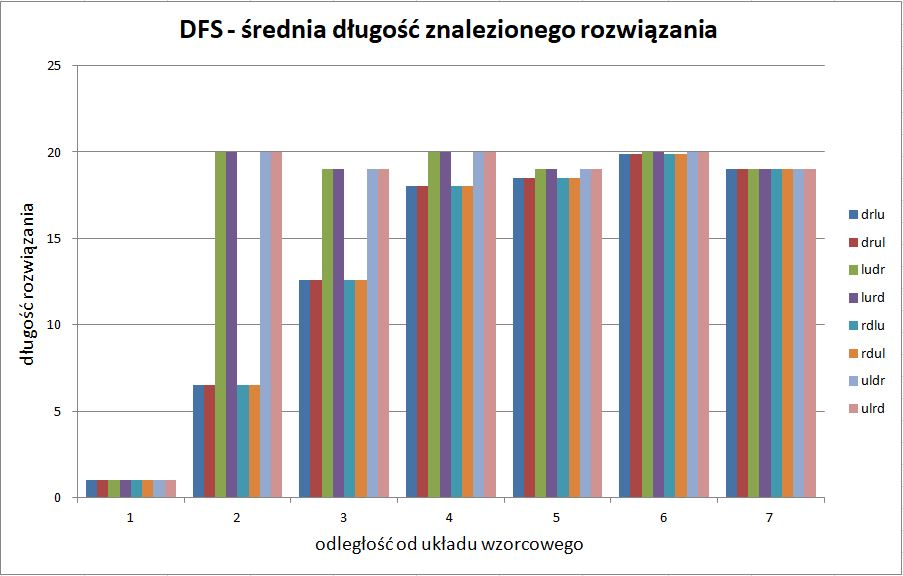
\includegraphics[scale=0.6]{dfs1}
		\caption{DFS - średnia długość znalezionego rozwiązania}
	\end{center}
\end{figure}
\newpage
\begin{figure}[ht!]
	\begin{center}
		\vspace{0.3in}
		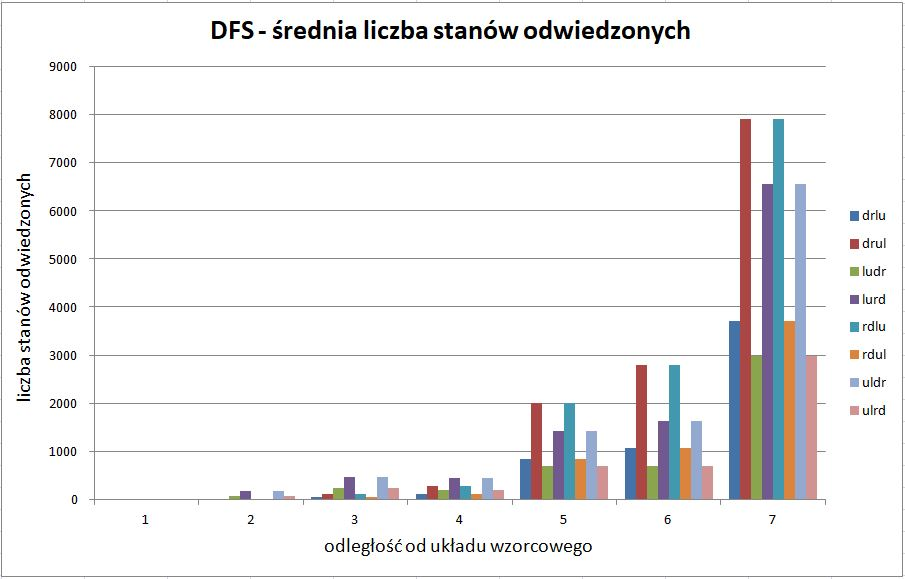
\includegraphics[scale=0.6]{dfs2}
		\caption{DFS - średnia liczba stanów odwiedzonych}
		\vspace{0.5in}
		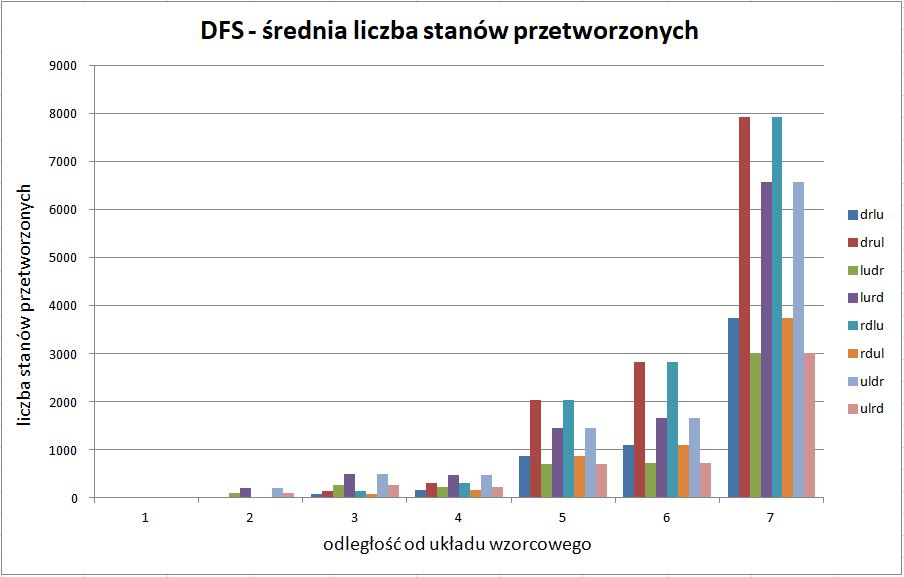
\includegraphics[scale=0.6]{dfs3}
		\caption{DFS - średnia liczba stanów przetworzonych}
	\end{center}
\end{figure}
\newpage
\begin{figure}[ht!]
	\begin{center}
		\vspace{0.3in}
		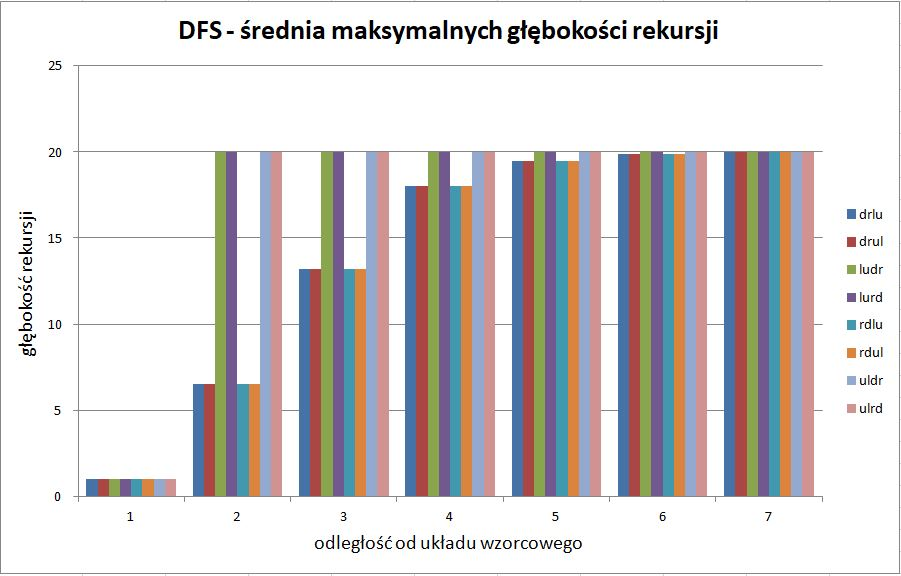
\includegraphics[scale=0.6]{dfs4}
		\caption{DFS - średnia maksymalnych głębokości rekursji}
		\vspace{0.5in}
		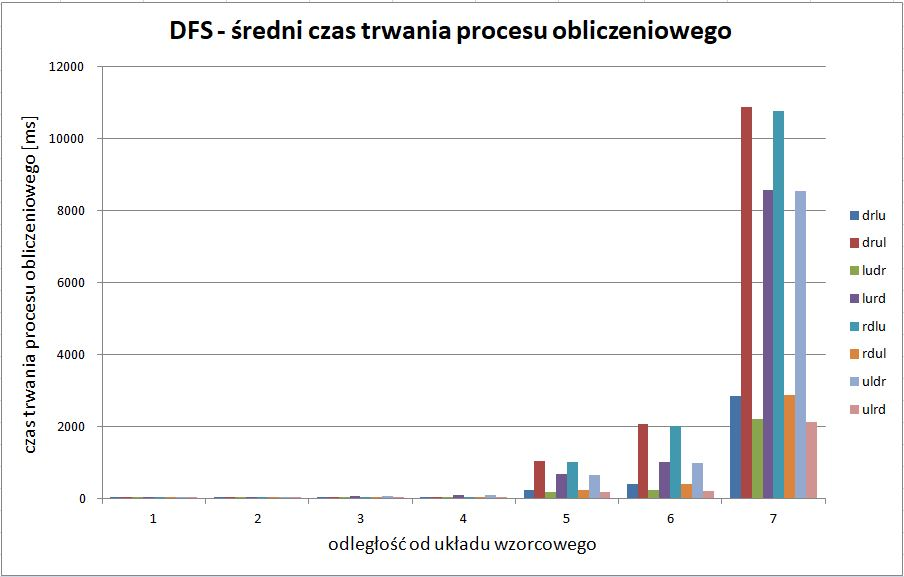
\includegraphics[scale=0.6]{dfs5}
		\caption{DFS - średni czas trwania procesu obliczeniowego}
	\end{center}
\end{figure}
\newpage
\begin{figure}[ht!]
	\begin{center}
		\vspace{0.3in}
		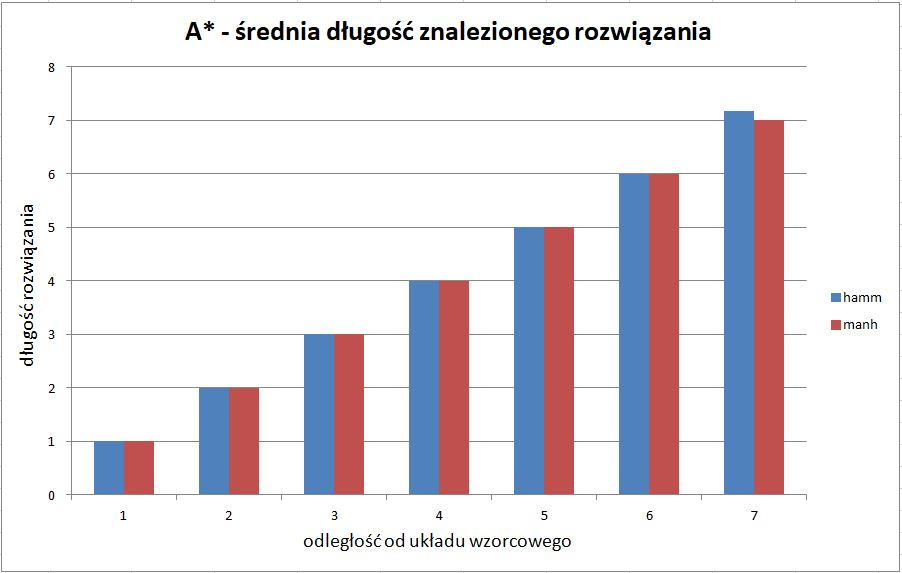
\includegraphics[scale=0.6]{astr1}
		\caption{A* - średnia długość znalezionego rozwiązania}
		\vspace{0.5in}
		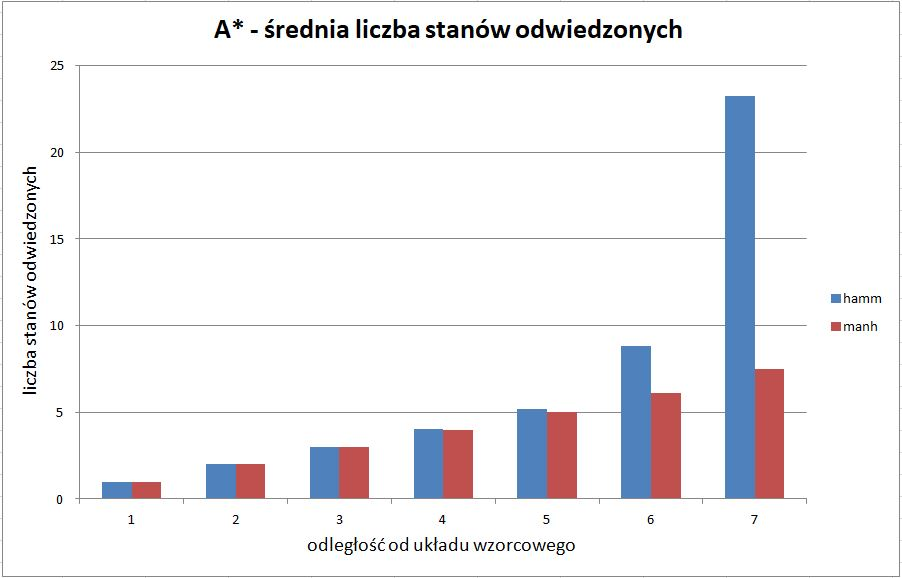
\includegraphics[scale=0.6]{astr2}
		\caption{A* - średnia liczba stanów odwiedzonych}
	\end{center}
\end{figure}
\newpage
\begin{figure}[ht!]
	\begin{center}
		\vspace{0.3in}
		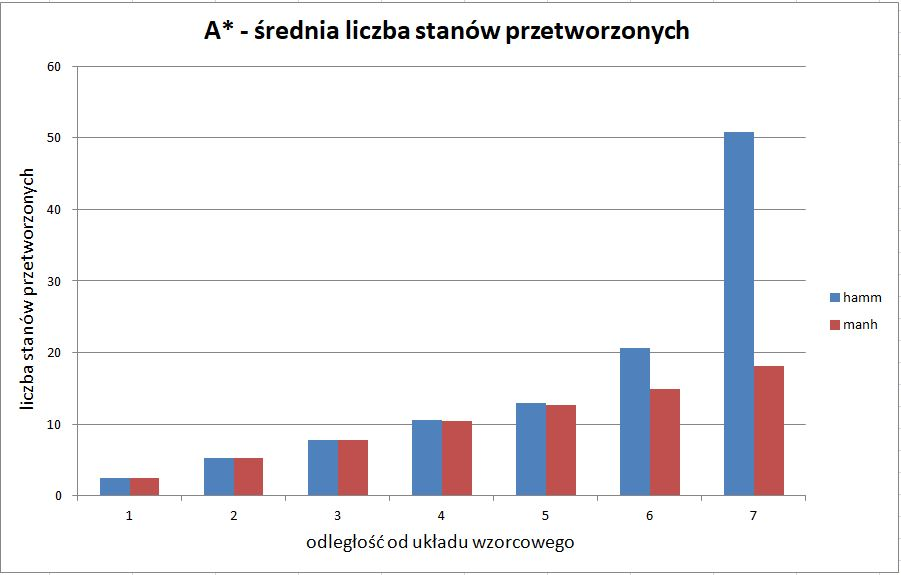
\includegraphics[scale=0.6]{astr3}
		\caption{A* - średnia liczba stanów przetworzonych}
		\vspace{0.5in}
		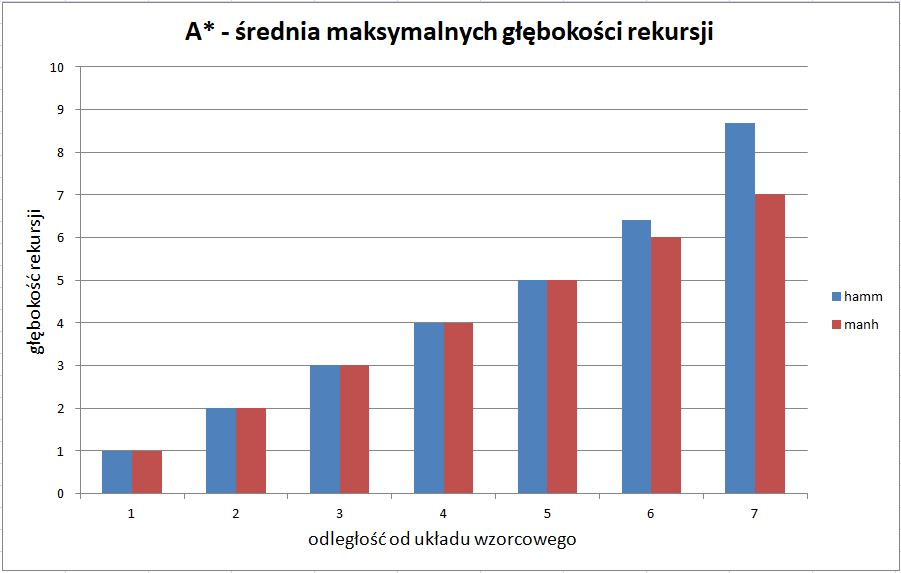
\includegraphics[scale=0.6]{astr4}
		\caption{A* - średnia maksymalnych głębokości rekursji}
	\end{center}
\end{figure}
\newpage
\begin{figure}[ht!]
	\begin{center}
		\vspace{0.3in}
		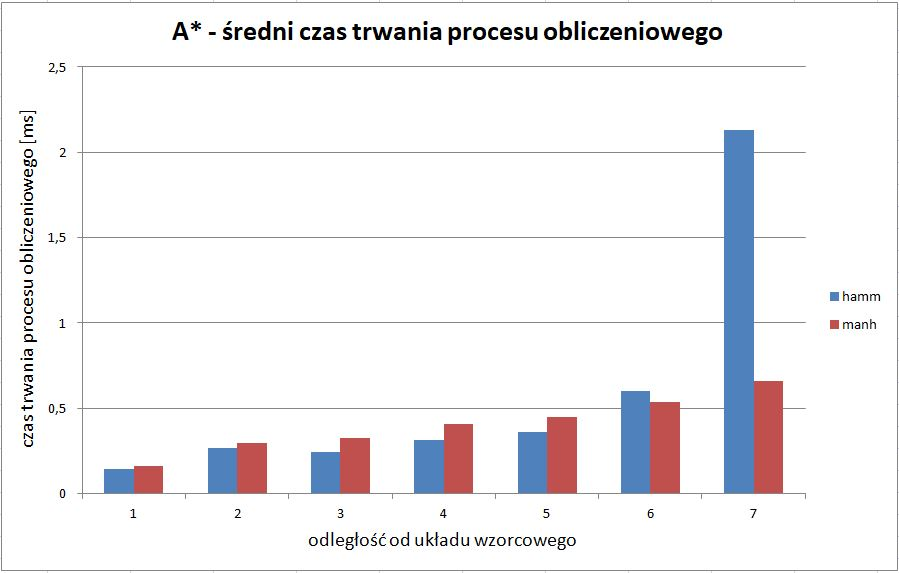
\includegraphics[scale=0.6]{astr5}
		\caption{A* - średnia czas trwania procesu obliczeniowego}
	\end{center}
\end{figure}

}

\section{Dyskusja}
\subsection{BFS}
{\color{black}
W oparciu o wykres przedstawiający średnią długość znalezionego rozwiązania można zauważyć, że niezależnie od wybranego porządku przeszukiwania sąsiedztwa wyniki są takie same. A dokładniej - równe odległości od układu wzorcowego. Średnia liczba stanów odwiedzonych jest natomiast zależna od wspomnianego wcześniej porządku przeszukiwania. Liczba stanów odwiedzonych, w znacznej większości jest wyższa dla porządków ludr, lurd, uldr oraz ulrd niż dla pozostałych. Wyjątek stanowią układy o odległości od układu wzorcowego równej 7 – tutaj sytuacja jest odwrotna oraz dla odległości równej 6, gdzie liczba stanów przetworzonych jest taka sama dla każdego z porządków. Warto zauważyć, że wraz ze wzrostem odległości od układu wzorcowego, parabolicznie rośnie średnia liczba stanów odwiedzonych. To samo zjawisko można zauważyć na wykresie przedstawiającym średnią liczbę stanów przetworzonych. Analizując wykres średniej maksymalnych głębokości rekursji można dojść do wniosku, że wyniki są niezależnie od porządku przeszukiwania i jednocześnie równe odległości od układu wzorcowego. Ze wzrostem odległości od układu wzorcowego proporcjonalnie rośnie wartość głębokości rekursji – identycznie jak w przypadku średniej długości rozwiązania. 
Z danych zawartych na wykresie przedstawiającym średni czas trwania procesu obliczeniowego nie da się jednoznacznie odnaleźć zależności między czasem a porządkami przeszukiwania. Da się natomiast zauważyć, że im większa jest odległość od układu wzorcowego tym więcej czasu algorytm potrzebuje na znalezienie prawidłowego rozwiązania. Różnice w czasie są niewielkie dla odległości 
z zakresu 1 – 3. Największa różnica zauważalna jest dla odległości równych 6 oraz 7.}

\subsection{DFS}
{\color{black}
W oparciu o wykres przedstawiający średnią długość znalezionego rozwiązania można zauważyć, że dla porządków przeszukiwania ludr, lurd, uldr oraz ulrd prawie zawsze wartości mieszczą się 
w zakresie 18 – 20. Wyjątkiem są układy o odległości od układu wzorcowego równej 1. Analizując wykres można zauważyć, że znalezione przez algorytm rozwiązania znacznie różnią się od możliwie najkrótszych. Średnia liczba stanów odwiedzonych oraz przetworzonych dla algorytmu DFS jest największa przy zastosowaniu porządków drul oraz rdlu, a następnie dla lurd oraz uldr. Patrząc dalej na wykresy, można zaobserwować znaczny wzrost liczby stanów między układami o odległości od układu wzorcowego równej 6, a tymi o odległości równej 7. Odnosząc się do wykresu przedstawiającego średnią maksymalnych głębokość rekursji można zaobserwować, że dla wszystkich układów, oprócz tych o odległości równej 1, porządki przeszukiwań ludr, lurd, uldr oraz ulrd zawsze osiągały wartość równą 20. Pozostałe porządki przeszukiwań uzyskiwały podobną wartość dopiero dla układów o odległości od układu wzorcowego równej 4 i więcej. Średni czas trwania procesu obliczeniowego dla każdego z porządku przeszukiwań rośnie około 5 krotnie między odległościami 
6 i 7. Najmniej czasu na znalezienie prawidłowego rozwiązania potrzebował algorytm korzystając 
z porządków przeszukiwania ludr oraz ulrd.}

\subsection{A*}
{\color{black}
W oparciu o wykres przedstawiający średnią długość znalezionego rozwiązania można zauważyć, że wybór wykorzystywanej metryki nie ma zbyt dużego znaczenia. Różnica dotyczy tylko układów 
o odległości od układu wzorcowego równej 7 i jest bardzo niewielka. Dodatkowo można zaobserwować, że odległość od układu wzorcowego jest wprost proporcjonalna do długości rozwiązania. Różnica liczby stanów odwiedzonych dla poszczególnych metryk rośnie wraz ze wzrostem odległości od układu wzorcowego. Dla metryki Manhattan wraz ze wzrostem odległości od układu wzorcowego ilość stanów odwiedzonych zwiększa się o bardzo zbliżoną wartość (1 – 1,30). Dla metryki Hamminga natomiast, wartość ta rośnie parabolicznie. Podobną sytuację można zauważyć na wykresie przedstawiającym średnią liczbę stanów przetworzonych. Jednakże różnica między metrykami w ilości stanów przetworzonych wraz ze wzrostem odległości od układu wzorcowego jest znacznie większa niż w przypadku stanów odwiedzonych. Widoczne jest to szczególnie dla odległości równych 6 i 7. W pierwszym przypadku (stany odwiedzone) różnice wynosiły odpowiednio 2,80 i 15,76. W drugim przypadku (stany przetworzone) różnice wynosiły odpowiednio 5,66 i 32,67. Średnia maksymalnej głębokości rekursji różni się dla obu metryk dla układów o odległości od układu wzorcowego większej niż 5. Widać wyraźnie, że dla metryki Hamminga wartość ta jest większa, jednakże różnice są niewielkie (0,41 – 1,67). Średni czas trwania procesu obliczeniowego jest mniejszy dla metryki Hamminga przy układach o odległości z zakresu 1 – 5. Dla odległości równej 6 oraz 7 średni czas jest mniejszy dla metryki Manhattan.}

\section{Wnioski}
{\color{black}
\begin{itemize}
  \item Dla algorytmu A* i BFS średnia długość znalezionego rozwiązania rośnie liniowo do odległości badanego układu od układu wzorcowego, dla algorytmu DFS jest to wartość znacznie wyższa, w większości przypadków zbliżona do maksymalnej głębokości rekursji ustalonej w zadaniu,
  \item Średnia ilość stanów odwiedzonych i przetworzonych jest zdecydowanie mniejsza dla algorytmu A*, w porównaniu do algorytmów DFS i BFS,
  \item Dla algorytmu BFS i DFS średni czas potrzebny do znalezienia rozwiązania rośnie wykładniczo wraz ze wzrostem odległości badanego układu od układu wzorcowego,
  \item W każdym z rozpatrywanych kryteriów najgorsze wyniki uzyskano przy wykorzystaniu algorytmu DFS, przez co nie jest on dobrym wyborem przy rozwiązania problemu zadania,
  \item Najlepsze wyniki przy rozwiązywaniu problemu postawionego w zadaniu okazał się się być algorytm A* z metryką Manhattan,
  \item Algorytmy heurystyczne takie jak A* w większości przypadków pozwalają znaleźć rozwiązanie szybciej niż algorytmy bazujące na taktyce "brute-force". \newline
\end{itemize}}

\begin{thebibliography}{0}
  \bibitem{l2short} T. Oetiker, H. Partl, I. Hyna, E. Schlegl.
    \textsl{Nie za krótkie wprowadzenie do systemu \LaTeX2e}, 2007, dostępny
    online.
  \bibitem{l2short} Jerzy Wałaszek\\
    \url{https://eduinf.waw.pl/inf/alg/001_search/0110.php}
  \bibitem{l2short} Wikipedia wolna encyklopedia\\
    \url{https://en.wikipedia.org/wiki/Breadth-first_search}
  \bibitem{l2short} Wikipedia wolna encyklopedia\\
    \url{https://en.wikipedia.org/wiki/Depth-first_search}
  \bibitem{l2short} Wikipedia wolna encyklopedia\\
    \url{https://en.wikipedia.org/wiki/A*_search_algorithm}
  \bibitem{l2short} geeksforgeeks - jitt, akshitajp\\
    \url{https://www.geeksforgeeks.org/check-instance-15-puzzle-solvable/}
  \bibitem{l2short} algorytm.edu.pl\\
    \url{http://www.algorytm.edu.pl/grafy/przeszukiwanie-w-glab.html}
  \bibitem{l2short} cs.princeton.edu\\
    \url{https://www.cs.princeton.edu/courses/archive/fall12/cos226/assignments/8puzzle.html}
\end{thebibliography}

\end{document}
